\begin{figure}[tb]
\centering
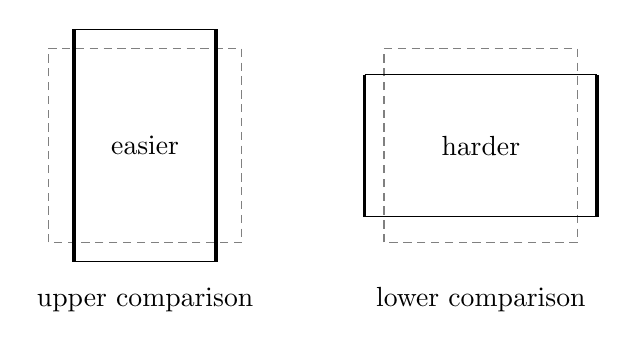
\begin{tikzpicture}[scale=.82]
 \begin{scope}
  \draw[densely dashed,gray] (0,0) rectangle (3,3);
  \draw (0.4,-.3) -- (2.6,-.3) (0.4,3.3) -- (2.6,3.3);
  \draw[very thick] (0.4,-.3) -- (0.4,3.3)
                   (2.6,-.3) -- (2.6,3.3);
  \node at (1.5,1.5) {easier};
  \node[below] at (1.5,-.55) {upper comparison};
 \end{scope}
 \begin{scope}[xshift=5.2cm]
  \draw[densely dashed,gray] (0,0) rectangle (3,3);
  \draw (-.3,.4) -- (3.3,.4) (-.3,2.6) -- (3.3,2.6);
  \draw[very thick] (-.3,.4) -- (-.3,2.6)
                   (3.3,.4) -- (3.3,2.6);
  \node at (1.5,1.5) {harder};
  \node[below] at (1.5,-.55) {lower comparison};
 \end{scope}
\end{tikzpicture}
\caption{The Jordan-quad comparison in Schoenflies coordinates.
The dashed square is the limiting target; thick sides are separately
wired electrodes.  The easier quad extends beyond the free sides and
ends inside the target's electrode sides.  The harder quad has the
opposite inclusions.  Physical test polygons retain strict margins
after pullback and lattice approximation.}
\label{jordan:sandwich-figure}
\end{figure}
